\section{Lógica y Cálculo Proposicional}


    Muchos algoritmos y demostraciones usan expresiones lógicas tales como
    \texttt{si p entonces q}. Entonces es necesario conocer los casos en los cuales esas expresiones son \texttt{ciertas} o \texttt{falsas}. Discutiremos esto en esta unidad. 

    Tambi\'en investigamos el valor de verdad de enunciados cuantificados, que son aquellos que usan los cuantificadores lógicos \texttt{para todo...} y \texttt{existe...}
    \marginnote{    	En este curso, usaremos el \emph{sistema algebráico de computo} \texttt{SageMath}, el cuál está escrito con base en el lenguaje de programación \texttt{Python} e incorpora diversos paquetes de \texttt{OpenSource}.  
    	Puede acceder a este sistema, a trav\'es de \href{https://cloud.sagemath.com/}{https://cloud.sagemath.com/} }


\subsection{Proposiciones y Declaraciones Compuestas}

    Una proposición es un enunciado declarativo que puede ser cierto o falso, pero no ambos. 

    \begin{problema}
        ?`Cuál de los siguientes enunciados es una proposición?
        \begin{multicols}{2}
            \begin{enumerate}
                \item El hielo flota en el agua.
                \item China está en Europa.
                \item $2+2=4$
                \item $2+2=5$
                \item ?`A donde vas?
                \item Haz tu tarea.
            \end{enumerate}
        \end{multicols}
    \end{problema}
    


\subsection{Proposiciones compuestas}


    Muchas proposiciones están \texttt{compuestas} de proposiciones más simples, llamadas \emph{subproposiciones}, por medio de \emph{conectores lógicos.}  Una proposición se dice que es \emph{primitiva} si no puede descomponerse en proposiciones más simples.



    Por ejemplo, las siguientes proposiciones son compuestas
    \begin{itemize}
        \item ``Las rosas son rojas y las violetas son azules''
        \item ``Juan es inteligente y estudia hasta muy noche''
    \end{itemize}
    



    La propiedad fundamental de una proposición compuesta es que su valor de verdad está completamente determinado por los valores de verdad de sus subproposiciones y la manera en la cual están conectadas para formar la proposición compuesta. 


\subsection{Operaciones Lógicas Básicas}


    En esta sección discutiremos las tres operaciones lógicas básicas: conjunción , disyunción  y la negación.


\subsection{Conjunción $p \wed q$}


    Cualesquiera dos proposiciones $p,q$ pueden ser combinadas por la palabra ``y'' para formar una proposición compuesta llamada \emph{conjunción} que se escribe $p\wed q.$



    \begin{defn}
        Si tanto $p$ como $q$ son ciertas, entonces $p \wed q$ es cierta; en otro caso $p\wed q$ es falsa.
        \sidenote{
        	\begin{tdv}[Conjunción]\hfill
        		\label{tdv:and}
        		\begin{center}
        			\begin{tabular}{|l|l|l|}\hline
        				$p$ & $q$ & $p \wed q$\\\hline
        				1 & 1 & 1\\\hline
        				1 & 0 & 0\\\hline
        				0 & 1 & 0\\\hline
        				0 & 0 & 0\\\hline
        			\end{tabular}
        		\end{center}        
        	\end{tdv}
        }  
    \end{defn}	

    \begin{rem}
        Para entender mejor como se conectan los valores de verdad, generalmente se utilizan \emph{tablas de verdad.}  
        
        Por brevedad $1$ representará el valor \texttt{cierto}, mientras que $0$ representará \texttt{falso}
    \end{rem}
    
    	\marginnote{
    	Construimos la tabla de verdad de la conjunción en el siguiente script \href{https://cloud.sagemath.com/projects/12787063-cafe-4f3b-a2e0-905f8b83cf3b/files/MD01_TRDV01_AND.sagews}{https://goo.gl/hEF5os}
    }

\subsection{Disyunción $p \vee q$}


    Cualesquiera dos proposiciones $p,q$ pueden ser combinadas por la palabra ``o'' para formar una proposición compuesta llamada \emph{disyunción} que se escribe $p \vee q .$



    \begin{defn}
        Si tanto $p$ como $q$ son falsas, entonces $p \vee q$ es falsa; en otro caso $p\vee q$ es verdadera.
        \sidenote{
        \begin{tdv}[disyunción] \hfill
    	\label{tdv:or}
    	\begin{center}
    		\begin{tabular}{|l|l|l|}\hline
    			$p$ & $q$ & $p \vee q$\\\hline
    			1 & 1 & 1\\\hline
    			1 & 0 & 1\\\hline
    			0 & 1 & 1\\\hline
    			0 & 0 & 0\\\hline
    		\end{tabular}
    	\end{center}
    	
    \end{tdv}    
    }
    \end{defn}
\marginnote{
Construimos la tabla de verdad de la disyunción en el siguiente script \href{https://cloud.sagemath.com/projects/12787063-cafe-4f3b-a2e0-905f8b83cf3b/files/MD01_TDV02_OR.sagews}{https://goo.gl/5kXzNI} 
}
 \begin{rem}
  Algunas veces \texttt{``p o q''} se entiende en el sentido exclusivo: Puede ocurrir \texttt{p} o \texttt{q}, \emph{pero no ambos,} que es diferente a la definición anterior. Sin embargo, existe un conector llamado de hecho \texttt{o exclusivo,} que cumple esta definición y consideraremos más adelante. 
 \end{rem}



\subsection{Negación $\neg p$}


 Dada cualquier proposición $p,$ otra proposición llamada \emph{negación} de $p$ puede ser formada escribien \emph{``No es cierto que...''} o \emph{``Es falso que...''} antes de \texttt{p}.
 
 De manera más sencilla, decimos \texttt{no $p$} y escribimos $\neg p.$
 
\begin{defn}[Negación]
 Si $p$ es cierta, entonces $\neg p$ es falsa; pero si $p$ es falsa, $\neg p$ es cierta.
 \sidenote{
    \begin{tdv}[Negación] \hfill
	\label{tdv:not}
	\begin{center}
		\begin{tabular}{|l|l|}\hline
			$p$ & $\neg p$\\\hline
			1 & 0 \\\hline
			0 & 1 \\\hline
		\end{tabular}
	\end{center}
	
\end{tdv} 
}
\end{defn}
\marginnote{
    Construimos la tabla de verdad de la disyunción en el siguiente script \href{https://cloud.sagemath.com/projects/12787063-cafe-4f3b-a2e0-905f8b83cf3b/files/MD01_TDV03_NOT.sagews}{https://goo.gl/sgCfkC}
}
\subsection{Proposiciones y Tablas de Verdad}

 Sea $P(p,q,...)$ una expresión construida con variables lógicas $p,q,...,$ que toman valores de \texttt{verdadero ``V''} o \texttt{falso ``F''}, a trav\'es de conectores lógicos como $\wed, \, \vee, \, \neg$ y otros  que discutiremos más adelante.
 
 Tales expresiones $P(p,q,...)$ son llamadas \emph{proposiciones.}

 La propiedad principal de una proposición $P(p,q,...)$ es que sus valores de verdad sólo dependen del valor de sus variables. 
 
 Una manera simple y concisa de mostrar esta relación es a trav\'es de una \emph{tabla de verdad.}

 \begin{problema}
  Contruir la tabla de verdad de la proposición
  $\neg \left( p \wed \neg q \right).$
\begin{solucion}
	   \begin{tdv}[$\neg\left( p \wed \neg q \right)$]
		
		\hfill
		\begin{center}
			\begin{tabular}{lllll}
				p & q & not q & p and not q & not( p and not q) \\
				$1$ & $1$ & $0$ & $0$ & $1$ \\
				$1$ & $0$ & $1$ & $1$ & $0$ \\
				$0$ & $1$ & $0$ & $0$ & $1$ \\
				$0$ & $0$ & $1$ & $0$ & $1$ \\
			\end{tabular}
		\end{center}
	\end{tdv}
\end{solucion}
 \end{problema} \marginnote{ Construimos la tabla de verdad de la proposición anterior con el siguiente script \href{https://goo.gl/V2Axzi}{https://goo.gl/V2Axzi}}


\marginnote{
 \begin{rem}
	Para evitar el uso excesivo de paréntesis, algunas veces adoptamos una jerarquía para los conectores lógicos. 
	
	
	De manera especifica $\neg$ tiene prioridad sobre $\wed,$ que a su vez tiene prioridad sobre $\vee$.
	
	
	
	Por ejemplo, $\neg p \wed q$ significa $\left( \neg p \right) \wed q$  y no
	$ \neg(p \wed q).$
	
	
\end{rem}
}

 \subsection{M\'etodo alternativo de construir una tabla de verdad}
\begin{center}
\begin{tabular}{|l|l|l|l|l|l|l|}\hline
 $p$ & $q$ & $\neg$ & $(p$ & $\wed$ & $\neg$ & q) \\\hline
 $1$ & $1$ &  &  & &  & \\\hline
 $1$ & $0$ &  &  & &  & \\\hline
 $0$ & $1$ &  &  & &  & \\\hline
 $0$ & $0$ &  &  & &  & \\\hline
\end{tabular}
\end{center}




\begin{problema} Construya las tablas de verdad de las siguientes proposiciones
\begin{enumerate}
 \item $p\vee \neg p$
 \item $p\wed \neg p$
 \item $\neg\left( p \vee q \right)$
 \item $\neg p \wed \neg q$
 \item $\neg\left( p \wed q \right)$
 \item $\neg p \vee \neg q$
\end{enumerate}


\end{problema}


 Algunas proposiciones $P(p,q,...)$ son siempre ciertas, no importa los valores de verdad de las variables $p,q,...$ 
  
 
 Tales proposiciones se conocen como \emph{tautologías.}



 De manera similar, algunas proposiciones $P(p,q,...)$ son siempre falsas, no importa los valores de verdad de las variables $p,q,...$ 
  
 
 Tales proposiciones se conocen como \emph{contradicciones.}






\subsection{Equivalencias Lógicas}


 Diremos que dos proposiciones $P(p,q,...)$ y $Q(p,q,...)$ son \emph{lógicamente equivalentes} si tienen tablas de verdad identidades. 
 
 
 En tal caso, escribimos $$P(p,q,..)\equiv Q(p,q,...)$$



 \begin{problema} Demostremos que 
  $$
  \neg\left( p \wed q \right) \equiv \neg p \vee \neg q
  $$
 \end{problema}




 \begin{problema}
  Reescriba la frase ``No es cierto que: las rosas son rojas y las violetas son azules'', usando la equivalencia anterior.
 \end{problema}



%\subsection{álgebra de proposiciones}


 Por su utilidad, algunas equivalencias lógicas con llamadas \emph{leyes para el álgebra de proposiciones.}
 
 
 A continuación, enunciaremos algunas, pero es necesario verificar su validez a trav\'es de tablas de verdad. 



% TODO: \usepackage{graphicx} required
\begin{figure}
	\centering
	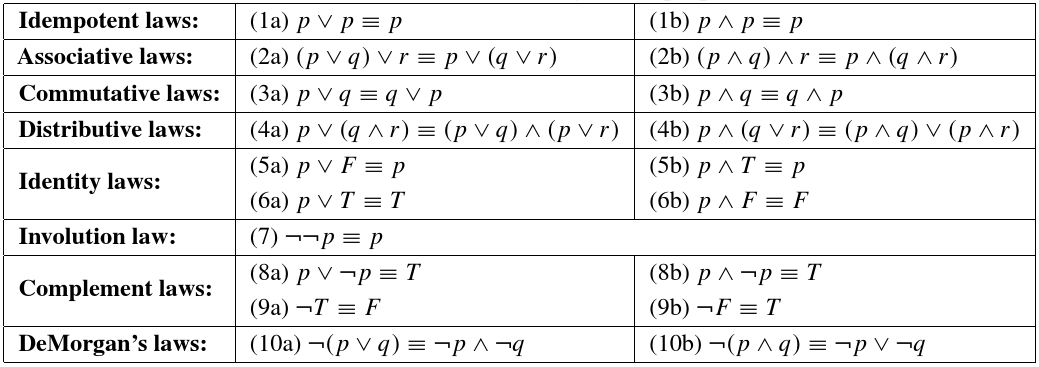
\includegraphics[width=\linewidth]{md/tabla_4-1}
 \caption{Leyes para el álgebra de proposiciones}
\label{fig:tabla:4.1}
\end{figure}



\subsection{Sentencias condicionales y bicondicionales}


 Muchas sentencias, particularmente en matemáticas, son de la forma \texttt{``si $p$ entonces $q$''}.  Tales sentencias son llamadas \emph{condicionales} y son denotadas por 
 $$
 p \imply q.
 $$ 



 El condicional $p \imply q$ es frecuentemente leído como \emph{``$p$ implica $q$''} o \emph{``$p$ sólo si $q$''.}
 \sidenote{
 \begin{tdv}[Condicional]
	\begin{center}
		\begin{tabular}{|l|l||l|} \hline
			$p$ & $q$ & $p \imply q$ \\ \hline
			$1$ & $1$ & $1$ \\ \hline
			$1$ & $0$ & $0$ \\ \hline
			$0$ & $1$ & $1$ \\ \hline
			$0$ & $0$ & $1$ \\ \hline
		\end{tabular}
	\end{center}
	
\end{tdv} 
}



 Otra sentencia común es de la forma \emph{``$p$ si y solo si $q$''.}  Tales sentencias son llamadas \emph{bicondicionales} y se denota por 
 $
 p \iff q.
 $ \sidenote{ 
 \begin{tdv}[Bicondicional]
	\begin{center}
		\begin{tabular}{|l|l||l|} \hline
			$p$ & $q$ & $p \biconditional q$ \\ \hline
			$1$ & $1$ & $1$ \\ \hline
			$1$ & $0$ & $0$ \\ \hline
			$0$ & $1$ & $0$ \\ \hline
			$0$ & $0$ & $1$ \\ \hline
		\end{tabular}
	\end{center}
	
\end{tdv} 
}







 \begin{problema}
  Demuestre que $$p\imply q \equiv \neg p \vee q.$$
 \end{problema}




 \begin{problema} Determine cuales de las siguientes sentencias son tautologías, construyendo las correspondientes tablas de verdad.
  \begin{enumerate}
   \item $\neg\left( p \vee \neg q \right) \imply \neg p$
   \item $p \imply \left( q\imply r \right)$
   \item $\left( p \imply q \right)\imply r$
   \item $\left( p\imply q \right) \imply \left( q\imply p \right)$
   \item $\left( p \wed \left( p \imply q \right) \right) \imply q$
   \item $\left( p \wed q \right) \imply p$
   \item $q \imply \left( \neg p \vee \neg q \right)$
   \item $\left( \left( p\imply q \right) \wed \left( q \imply r \right) \right) \imply \left( p \imply r \right)$
  \end{enumerate}

 \end{problema}



\subsection{Argumentos}


 Un \emph{argumento} es una afirmación de que un conjunto dado de proposiciones $$P_{1}, P_{2},...,P_{n},$$ llamadas \emph{premisas}, tiene como consecuencia otra proposición $Q,$ llamada \emph{conclusión.}\sidenote{
Por ejemplo
  \begin{center}
	\begin{tabular}{l}
		Si sube el dólar, sube la gasolina.\\
		Si sube la gasolina, entonces hay inflación.\\\hline
		$\therefore$ Si sube el dólar, entonces hay inflación.
	\end{tabular}
\end{center} 
}
 
 En otras palabras, es una sentencia de la forma
 $$
  \left( P_{1} \wed P_{2} \wed...\wed P_{n}\right) \imply Q
  $$
 
 
 
 Tal argumento se denota por $$P_{1}, P_{2},...,P_{n} \yields Q.$$



 La noción de \emph{``argumento lógico''} o \emph{``argumento válido''} se formaliza de la manera siguiente:
 
 
 \begin{defn}
  \label{lip:4.4}
  Un argumento $P_{1}, P_{2},...,P_{n} \yields Q$ se dice que es \emph{válido} si la proposición 
  $$
  \left( P_{1} \wed P_{2} \wed...\wed P_{n}\right) \imply Q
  $$ es una tautología.
  
   Si un argumento no es \emph{válido,} diremos que es una \emph{falacia.}
 \end{defn}




 \begin{problema}
 \label{lip:exmp:4.4}
  \begin{enumerate}
   \item Demuestre que $p, p\imply q \yields q$ es un argumento válido. 
   \item Demuestre que $p\imply q, q \yields p$ es una falacia.
   
   \item Demuestre que $p\imply q, \neg q \yields \neg p$ es un argumento válido.
  \end{enumerate}

 \end{problema}

	% TODO: \usepackage{graphicx} required
	\begin{figure}
		\centering
		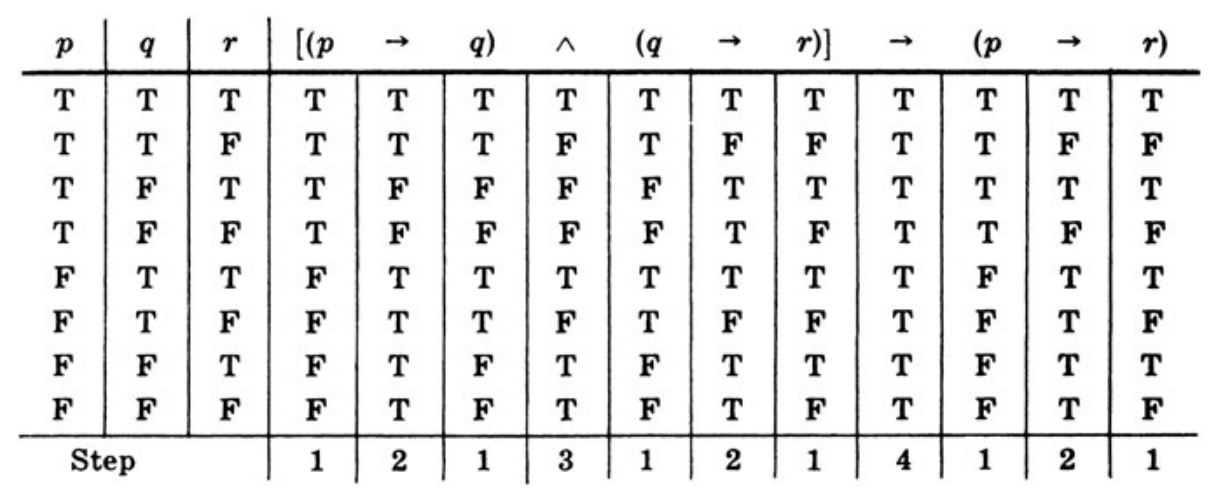
\includegraphics[width=0.7\linewidth]{md/tabla_silogismo}
		\caption{
			  Un principio fundamental del razonamiento lógico nos dice que:
				Si $p$ implica $q$ y $q$ implica $r,$ entonces $p$ implica $r.$ 
			En otras palabras, el siguiente argumento es válido
			$$
			p\imply,q, q\imply r \yields p \imply r.
			$$ }
		%\label{fig:tablasilogismo}
		\label{fig:tabla_silogismo}
	\end{figure}

\subsection{Funciones proposicionales y Cuantificadores}


 Una \emph{función proposicional} (o \emph{sentencia abierta} o \emph{condición}) definida en un conjunto $A$ es una expresión $p(x)$ que tiene la propiedad de que $p(a)$ es cierta o falsa para cada $a \in A.$



 El conjunto $A$ se conoce como dominio de $p(x),$ y el subconjunto de todos los elementos para los cuales $p(x)$ es cierto se conoce como el \emph{conjunto de verdad} $T_{p}$ de $p(x):$
 
 $$T_{p}=\set{x \mid x\in A, p(x)=\texttt{1}},$$ 
 o simplemente 
 $$
 T_{p}=\set{x \mid p(x)}.
 $$


\begin{defn}
	El conjunto de los números naturales está dado por
	\begin{equation} \N = \set{0,1,2,3...} .\end{equation}	
	
\end{defn}

 \begin{problema}
  \label{lip:exmp:4.7}
  Encuentre el conjunto de verdad para cada función en $\N$:
  \begin{enumerate}
   \item $p(x): x+2>7$ 
   \item $p(x): x+5<3$ 
   \item $p(x): x+5>1$ 
  \end{enumerate}

 \end{problema}



\subsection{Cuantificador universal}


 Sea $p(x)$ una función proposicional definido en un conjunto $A.$ La expresión
 \begin{equation}
 \label{lip:4.1}
   \forall x \in A: p(x)
 \end{equation} 
 se lee como  \texttt{``para todo $x\in A,$ $p(x)$ es verdadero.''}  
 
 El símbolo $\forall$ (\texttt{``para todo''}) se llama cuantificador universal.




 Mientras que $p(x)$ es una sentencia abierta (su valor de verdad depende de cada $x\in A$), la afirmación 
 $$\forall x\in A: p(x)$$ es verdadera si y solo si $p(x)$ se cumple para todo $x\in A.$  



 Por otro lado, si existe algún $x\in A$ tal que $p(x)$ es falso, entonces $$\forall x\in A: p(x)$$ es falso.



 \begin{problema}
  \label{lip:exmp:4.8}
  Verifique el valor de verdad de las siguientes afirmaciones:
  \begin{enumerate}
   \item $\forall n \in \N: n+4>3.$ 
   \item $\forall n \in \N: n+2>8.$
  \end{enumerate}

 \end{problema}



\subsection{Cuantificador existencial}


 Sea $p(x)$ una función proposicional definido en un conjunto $A.$ La expresión
 \begin{equation}
 \label{lip:4.3}
   \exists x \in A: p(x)
 \end{equation} 
 se lee como  \texttt{``existe $x\in A,$ tal que $p(x)$ es verdadero.''}  
 
 El símbolo $\exists$ (\texttt{``existe...''}) se llama cuantificador existencial.




 Mientras que $p(x)$ es una sentencia abierta (su valor de verdad depende de cada $x\in A$), la afirmación 
 $$\exists x\in A: p(x)$$ es verdadera si y solo si $p(x)$ se cumple para algún elemento $x\in A.$  



 Por otro lado,  $$\exists x\in A: p(x)$$ es falso si y solo si para todo $ x\in A $, se tiene que $ p(x) $ es falso.



 Verifique el valor de verdad de las siguientes afirmaciones:
 \begin{enumerate}
  \item $\exists n  \in \N: n+4<7;$ 
  \item $\exists n \in \N: n+6<4.$
 \end{enumerate}



\subsection{Negación de Sentencias Cuantificadas}



 Considere la afirmación:
 \begin{center}
  \emph{Todos los estudiantes de ingeniería saben programar.}
 \end{center}
?`Cómo podemos negar esta afirmación?


\begin{center}
 \emph{Al menos un estudiante de ingeniería no sabe programar.}
\end{center} 


 De manera similar, la negación de la afirmación
 \begin{center}
  \emph{Existe algún estudiante de ingeniería que sepa programar}
 \end{center}
 es equivalente a afirmar que 
 \begin{center}
  \emph{Cada uno de los estudiantes de ingeniería no saben programar.}
 \end{center}

Estos son ejemplos de la siguiente proposición

 \begin{thm}[DeMorgan]
  \begin{align}
  \label{lip:thm:4.4}
   \neg\left( \forall x\in M: p(x) \right)& \equiv \exists x\in M: \neg p(x)\\
   \label{lip:thm:4.5}
   \neg\left( \exists x\in M: p(x) \right)& \equiv \forall x\in M: \neg p(x).
  \end{align}

 \end{thm}




 \begin{ejemplo}
  \label{lip:exmp:4.10.a}
  La negación de la siguiente afirmación
  \begin{center}
   \emph{Para todo entero positivo $n,$ tenemos que $n+2>8$}
  \end{center}
es 
\begin{center}
 \emph{Existe un entero positivo $n$ tal que $n+2 \leq 8.$}
\end{center}

 \end{ejemplo}




 \begin{ejemplo}
  \label{lip:exmp:4.10.b}
  La negación de la siguiente afirmación
  \begin{center}
   \emph{Existe una persona viva con 150 a\~nos o más.}
  \end{center}
 es 
 \begin{center}
  \emph{Toda persona viva tiene menos de 150 a\~nos.}
 \end{center}

 \end{ejemplo}




\marginnote{ \begin{rem}
  Para negar una afirmación del tipo $$\forall x \in A: p(x)$$ sólo necesitamos encontrar un elemento $x_{0}\in A$ tal que $p(x)$ sea \emph{falso.}
  
  
  A un elemento $x_{0}$ así se le conoce como \emph{contraejemeplo.}
 \end{rem}}




 \begin{ejemplo}
 \label{lip:4.11}
  \begin{enumerate}[(a)]
   \item 
  Un contraejemplo para $\forall x \in \R: \abs{x}\neq 0$ es $x=0.$  
   \item 
  Un contraejemplo para $\forall x \in \R: x^{2}\geq x$ es $x=\frac{1}{2}.$  
   \item 
  Sin embargo, $\forall x \in \N: : x^{2}\leq x$ es siempre cierto.
  \end{enumerate}

 \end{ejemplo}



\subsection{Problemario}

%\subsection{Proposiones y Tablas de Verdad}


 \begin{problema}
  Sea $p:\texttt{``Hace frío''}$ y $q:\texttt{``Está lloviendo''.}$ Proponga un enunciado verbal simple que describa cada una de las siguientes proposiciones:
  \begin{enumerate}
   \item $\neg p;$
   \item $p \wed q;$
   \item $p \vee q;$
   \item $q \vee \neg p.$
  \end{enumerate}

 \end{problema}




 \begin{problema}
  Encuentre la tabla de verdad de $\neg p \wed q.$
 \end{problema}




 \begin{problema}
  Demuestre que la propisición 
  $$
  p \vee \neg \left( p\wed q \right)
  $$ es una tautología.
 \end{problema}




 \begin{problema}
  Muestre que las proposiciones $\neg\left( p \wed q \right)$ y $\neg p \vee \neg q$ son lógicamente equivalentes.
 \end{problema}




 \begin{problema}
  Use las leyes en la tabla \ref{fig:tabla:4.1} para mostrar que 
  $$
  \neg \left( p \wed q \right) \vee \left( \neg p \wed  q \right) \equiv \neg p
  $$
 \end{problema}



%\subsection{Sentencias condicionales}


 \begin{problema}
  \label{lip:sol:4.6}
  Reescriba los siguientes enunciados sin usar el condicional:
  \begin{enumerate}
   \item Si hace frío, el usa sombrero. 
   \item Si la productividad se incrementa, entonces el salario aumenta.
  \end{enumerate}

 \end{problema}




 \begin{problema}
  \label{lip:sol:4.7}
  Considere la proposición condicional $p \imply q.$ La proposiciones 
  \begin{center}
  ${\color{red}q \imply p,} {\color{blue}\, \neg p \imply \neg q,} \, {\color{green}\neg q \imply \neg p}$
  \end{center}
son llamadas {\color{red} conversa,} {\color{blue}inversa} y {\color{green} contrapositiva}, respectivamente.


?`Cuáles de estas proposiciones son lógicamente equivalente s a $p\imply q$?
 \end{problema}




 \begin{problema}
  Determine la contrapositiva de cada enunciado:
  \begin{enumerate}
   \item Si Erik es poeta, entonces es pobre. 
   \item Solo si Marcos estudia, pasará el examen. 
  \end{enumerate}

 \end{problema}




 \begin{problema}
  Escriba la negación de cada enunciado, tan simple como sea posible:
  \begin{enumerate}
   \item Si ella trabaja, ganará dinero. 
   \item El nada si y solo si el agua está tibia. 
   \item Si neva, entonce no manejar\'e.
  \end{enumerate}

 \end{problema}



%\subsection{Argumentos}


 \begin{problema}
  Muestre que el siguiente argumento es una falacia:
 $$
 p\imply q, \neg p \yields \neg q.
 $$
 \end{problema}




 \begin{problema}
  Muestre que el siguiente argumento es válido:
 $$
 p\imply q, \neg q \yields \neg p.
 $$
 \end{problema}




\begin{problema}
  Muestre que el siguiente argumento siempre es válido:
 $$
 p \imply \neg q, r \imply q, r \yields \neg p.
 $$
\end{problema}




 \begin{problema}
  Determine la validez del siguiente argumento:
  \begin{center}
\begin{tabular}{l}
Si $7$ es menor que $4$, entonces $7$ no es número primo\\
$7$ no es menor que $4$\\\hline
$7$ no es número primo.
  \end{tabular}
  \end{center}

 \end{problema}




 \begin{problema}
  Determine la validez del siguiente argumento:
  \begin{center}
\begin{tabular}{l}
Si dos lados de un triángulo son iguales, entonces los respectivos ángulos opuestos son iguales\\
Dos lados de un triángulo no son iguales\\\hline
Los respectivos ángulos opuestos no son iguales.
  \end{tabular}
  \end{center}

 \end{problema}



%\subsection{Cuantificadores y Funciones Proposicionales}


 \begin{problema}
  Sea $A=\set{1,2,3,4,5}.$ Determine el valor de verdad de cada uno de los siguientes enunciados:
  \begin{enumerate}
   \item $\exists x \in A: x+3=10;$ 
   \item $\forall x \in A: x+3<10;$ 
   \item $\exists x \in A: x+3<5;$ 
   \item $\forall x \in A: x+3 \leq 7.$
  \end{enumerate}

 \end{problema}




  \begin{problema}
    Determine el valor de verdad de cada uno de las siguientes afirmaciones donde $U=\set{1,2,3}$ es el conjunto \emph{``universo''} (de referencia):
 \begin{enumerate}
  \item $\exists x \forall y: x^{2}< y+1;$ 
  \item $\forall x \exists y: x^{2}+y^{2}<12;$ 
  \item $\forall x \forall y: x^{2}+y^{3}<12.$
 \end{enumerate}

  \end{problema}




 \begin{problema}
  Encuentre la negación de cada una de las siguientes afirmaciones:
  \begin{enumerate}
   \item $\exists x \forall y: p(x,y);$ 
   \item $\forall x \forall y: p(x,y);$ 
   \item $\exists x \exists y \forall z: p(x,y,z).$
  \end{enumerate}

 \end{problema}




 \begin{problema}
  Sea $$p(x): x+2>5.$$ Indique cuando $p(x)$ es una función proposicional o no en cada uno de los siguientes conjuntos: 
  \begin{enumerate}
   \item $\N$ 
   \item $\Z^{-}=\set{-1,-2,-3,...}$ 
   \item $\mathbb{C}$
  \end{enumerate}

 \end{problema}




	\begin{problema}
	Niegue cada uno de las siguientes afirmaciones:
	\begin{enumerate}
		\item Todos los estudiantes viven en los dormitorios.
		\item A todos los estudiantes de ingeniería le gusta el futbol.
		\item Algunos estudiantes tienen 25 años o más.
	\end{enumerate}
	\end{problema}



\subsection{Bibliografía}
 Las notas de esta sección están basadas en el capítulo 4 \texttt{``Logic and Propositional Calculus''} del libro
 \begin{center}
  \texttt{Lipschutz, S. and Lipson, M.;\textbf{ Schaum's Outline of Discrete Mathematics;} McGraw-Hill, 3th Edition.}
 \end{center}
